\documentclass[conference]{IEEEtran}
\IEEEoverridecommandlockouts
% The preceding line is only needed to identify funding in the first footnote. If that is unneeded, please comment it out.
\usepackage[utf8]{inputenc}
\usepackage[T1]{fontenc}
\usepackage[brazilian]{babel}
\usepackage{cite}
\usepackage{amsmath,amssymb,amsfonts}
\usepackage{algorithmic}
\usepackage{graphicx}
\usepackage{booktabs}
\usepackage{textcomp}
\usepackage{xcolor}
\def\BibTeX{{\rm B\kern-.05em{\sc i\kern-.025em b}\kern-.08em
    T\kern-.1667em\lower.7ex\hbox{E}\kern-.125emX}}
\begin{document}

\title{Análise estrutural das comunidades no Twitter
brasileiro durante o ciclo eleitoral de 2022}

\author{\IEEEauthorblockN{Vinícius Pinho Galvão}
\IEEEauthorblockA{\textit{Graduando em Sistemas de informação} \\
\textit{UFMG} \\
Belo Horizonte, Brasil \\
viniciuspgalvao@hotmail.com}
\and
\IEEEauthorblockN{Eliane Cristina de Freitas Rocha}
\IEEEauthorblockA{\textit{Orientadora} \\
\textit{UFMG} \\
Belo Horizonte, Brasil \\
prof.elianecfr@gmail.com}
}

\maketitle

\section{Introdução}
O segundo turno da eleição presidencial de 2022 terminou com a vitória de Lula sobre Jair Bolsonaro pela margem mais estreita desde a redemocratização \cite{b_interian2023}. Pouco mais de dois meses depois, em 8 de janeiro de 2023, apoiadores de Bolsonaro invadiram e depredaram as sedes dos três poderes em Brasília, contestando o resultado das urnas. Os mesmos fatos que, para boa parte do país, representavam um ataque à democracia eram descritos por outra parcela como um ato legítimo de protesto. Não havia um vocabulário comum entre as duas leituras, nem um espaço onde elas se confrontassem. O 8 de janeiro foi o momento em que essa distância, acumulada ao longo de todo o ciclo eleitoral, ficou impossível de ignorar.

Esse descompasso entre leituras de um mesmo acontecimento é o problema que este trabalho busca caracterizar. A ideia de que o Brasil está dividido em dois é quase um consenso intuitivo, algo que se percebe no dia a dia muito antes de aparecer em qualquer estatística. O que é menos óbvio, e mais interessante de investigar, é a forma dessa divisão. Afirmar que existem dois grupos opostos é diferente de afirmar que esses grupos estão isolados um do outro, e é diferente ainda de afirmar que eles se comportam da mesma maneira. Duas comunidades podem coexistir trocando ataques e informação o tempo todo, ou podem se fechar em ambientes paralelos que quase não se tocam. São situações distintas, com consequências distintas, e a primeira tarefa deste trabalho é tornar essa distinção visível a partir da estrutura concreta das comunidades.

As redes sociais são onde boa parte dessas leituras se forma e circula, e o Twitter ocupa nesse cenário uma posição particular, por ser uma plataforma centrada em opinião e em reação ao noticiário. Cada usuário monta a própria linha do tempo a partir de quem decide seguir e do que decide amplificar, e a esse recorte se soma o que o algoritmo escolhe promover. O resultado é que duas pessoas expostas ao mesmo evento podem ter contato com versões quase opostas dele, sem nunca verem a versão alheia. A plataforma funciona ao mesmo tempo como espelho e como agente formador: reflete divisões que já existem na sociedade e, ao reforçá-las dia após dia, ajuda a produzi-las.

O custo desse fechamento vai além do desconforto de uma conversa pública fragmentada. A circulação de desinformação sobre a Covid-19 no Twitter oferece um exemplo concreto, e grave, do que está em jogo. Recuero, Soares e Zago \cite{b_recuero2021} analisaram a circulação de links sobre a pandemia e encontraram uma divisão assimétrica entre os grupos: de um lado, um ambiente em que a desinformação aparecia fortemente associada a veículos hiperpartidários e a plataformas como o YouTube; de outro, um ambiente em que predominavam veículos jornalísticos e institucionais. Os dois temas que mais se beneficiaram desse fechamento foram a defesa da hidroxicloroquina como tratamento e a resistência à vacinação, e em ambos os casos o conteúdo amplificado contrariava a evidência científica. Meta-análises de ensaios clínicos randomizados recentes não encontraram benefício da hidroxicloroquina no tratamento da Covid-19, e uma delas associou seu uso a aumento de mortalidade \cite{b_axfors2021, b_singh2020}. A vacinação, por outro lado, teve efeito oposto: estima-se que tenha evitado da ordem de 14 milhões de mortes no primeiro ano de aplicação em 185 países \cite{b_watson2022}. O que circulava no ambiente fechado, portanto, não era apenas uma versão alternativa dos fatos, mas a versão que a evidência posterior desmentiu. Quando a dieta informativa de um grupo se fecha em torno de fontes que reforçam umas às outras, o que entra ali deixa de ser confrontado com o que circula fora, e no caso da pandemia esse descompasso teve consequências mensuráveis em saúde pública.

O mesmo mecanismo pode ajudar a entender o caminho até o 8 de janeiro. Para quem acompanhava a eleição imerso em um feed onde praticamente todos apoiavam o mesmo candidato, a derrota nas urnas era difícil de conciliar com a realidade observada todos os dias. Vista de dentro dessa bolha, em que se vê falar quase só do próprio lado, a suspeita de fraude não soa como teoria da conspiração, e sim como a conclusão mais coerente diante do que se observa. Analisando a polarização no Twitter durante a eleição de 2022, Interian e Rodrigues \cite{b_interian2023} observaram um isolamento acentuado e assimétrico da comunidade de direita e levantaram a hipótese de que esse isolamento, somado à facilidade de comunicação coordenada dentro do grupo, possa ter influenciado os atos golpistas de 8 de janeiro. É aqui que o papel da rede como formadora de realidade deixa de ser apenas uma metáfora. A exposição repetida a uma só versão dos fatos não determina o que cada pessoa faz, mas ajuda a entender por que contestar um resultado legítimo pôde parecer, para parte dos envolvidos, uma reação justificada.

Este trabalho parte da hipótese de que essa divergência não nasceu pronta no 8 de janeiro. Ela foi construída ao longo do ciclo eleitoral, evento após evento, e a invasão das sedes dos poderes foi o ápice de um processo mais longo. Para investigar isso, propõe-se analisar não apenas o 8 de janeiro de forma isolada, mas também eventos anteriores que compõem o arco que leva até ele, observando como as comunidades políticas no Twitter se organizaram em torno de cada um e em que medida suas leituras se separaram. O objetivo é caracterizar a estrutura dessas comunidades a partir dos dados e, com base nessa caracterização, perguntar não só se o Brasil está dividido, mas como ele está dividido: se o problema central é a existência de dois campos opostos ou o grau em que cada campo se fecha ao outro, e se os dois lados dessa divisão têm de fato o mesmo formato. Há indícios, tanto na literatura quanto nos resultados deste trabalho, de que não têm. 

\section{Referencial Teórico e Trabalhos Correlatos}
Este capítulo situa o trabalho em relação à literatura em três frentes. A primeira apresenta os conceitos de câmara de eco e de polarização informacional que enquadram o problema. A segunda revisa os trabalhos que analisaram a polarização no Twitter político brasileiro, com atenção especial aos que tratam do mesmo período e do mesmo evento estudados aqui. A terceira detalha a fundamentação metodológica da rede de co-retweet, que é a principal ferramenta de análise deste trabalho.

\subsection{Câmaras de eco e polarização informacional}
A noção de que plataformas digitais favorecem o surgimento de ambientes informacionais homogêneos tem duas formulações próximas e frequentemente confundidas. Pariser \cite{b_pariser2011} descreveu o filter bubble como efeito da personalização algorítmica: ao aprender as preferências de cada usuário, os sistemas de recomendação passam a entregar predominantemente conteúdo alinhado a essas preferências, reduzindo o contato com o que destoa delas. Sunstein \cite{b_sunstein2001} tratou das câmaras de eco a partir de um mecanismo distinto, mais social que algorítmico: a tendência de pessoas com visões semelhantes a se agruparem e a reforçarem mutuamente suas posições, filtrando o que contraria o consenso interno do grupo. Os dois fenômenos operam juntos na prática. A personalização entrega mais do mesmo, e a dinâmica de grupo amplifica o que já está alinhado, de modo que o ambiente informacional de um usuário tende a se estreitar tanto pela ação da plataforma quanto pela sua própria escolha de quem seguir e do que amplificar.

Para este trabalho, o que interessa nesses conceitos não é a experiência individual de cada usuário, e sim a forma como eles se manifestam na estrutura coletiva da rede. Quando uma comunidade política consome e amplifica de maneira consistente um conjunto de fontes que outra comunidade ignora, a separação deixa de ser apenas uma diferença de opinião e passa a ser uma propriedade mensurável da rede de interações. É possível, então, perguntar quão fechada uma comunidade está em relação às demais, quanto de informação atravessa a fronteira entre grupos e se esse fechamento se distribui de forma simétrica entre os lados. Tratar a câmara de eco como uma propriedade estrutural, e não como uma hipótese sobre o que se passa na mente de cada usuário, é o que permite estudá-la com as ferramentas de análise de redes empregadas aqui.

\subsection{Polarização no Twitter político brasileiro}
A polarização política no Twitter brasileiro é um fenômeno bem documentado, com contribuição central do grupo de pesquisa de Raquel Recuero. Analisando a eleição presidencial de 2018, Soares, Recuero e Zago \cite{b_soares2019} identificaram a formação de dois grupos antagônicos a partir do padrão de retweets, com pouca interação entre si. Um achado importante desse trabalho é que a polarização não era simétrica: os dois lados não se comportavam como imagens espelhadas, e um deles se mostrava mais isolado e mais coeso que o outro. Essa assimetria reaparece em diferentes contextos e serve de ponto de referência para os resultados apresentados neste trabalho.

O estudo de Recuero, Soares e Zago \cite{b_recuero2021} sobre a circulação de desinformação a respeito da Covid-19 oferece uma caracterização mais detalhada dessa assimetria, agora do ponto de vista do conteúdo consumido por cada grupo. Os autores observaram que a dieta informativa dos dois lados era qualitativamente distinta. De um lado, um ambiente em que a desinformação se associava fortemente a veículos hiperpartidários e a plataformas como o YouTube. De outro, um ambiente ancorado em veículos jornalísticos e institucionais. Esse resultado é relevante para o presente trabalho por dois motivos. Primeiro, porque reforça que a separação entre comunidades não se reduz à oposição entre dois polos de tamanho e comportamento equivalentes. Segundo, porque sugere que comunidades de um mesmo campo podem se distinguir pelo registro do conteúdo que amplificam, uma distinção que a caracterização das comunidades deste trabalho poderá examinar em etapa posterior.

O trabalho mais próximo do que se desenvolve aqui é o de Interian e Rodrigues \cite{b_interian2023}, que analisaram a polarização no Twitter durante a eleição brasileira de 2022 a partir de um conjunto de mais de quinze milhões de tweets. Os autores construíram uma rede de retweets e detectaram três grandes comunidades, a maior de usuários de esquerda, uma segunda de veículos de imprensa e seus seguidores, e uma terceira de usuários de direita, que juntas reuniam a maior parte dos usuários da rede. O principal resultado do estudo é uma medida de quanto cada grupo contribui para a polarização geral da rede. Apesar de a comunidade de direita ser menor que a de esquerda, ela respondia, em média, por 44,1\% da modularidade da rede, contra 13,4\% da comunidade de esquerda. A comunidade de direita era, portanto, marcadamente mais isolada e mais coesa, e os autores levantam a hipótese de que esse isolamento, somado à facilidade de comunicação coordenada dentro do grupo, possa ter contribuído para os atos de 8 de janeiro de 2023.

Há, porém, uma diferença metodológica decisiva entre aquele trabalho e este. Interian e Rodrigues modelam uma rede de retweets dirigida, em que cada aresta liga o autor original de um tweet ao usuário que o retuitou e indica o sentido da propagação da informação. Construir essa rede exige conhecer o autor original de cada tweet retuitado. O dataset utilizado neste trabalho preserva apenas o identificador do tweet referenciado, e não o seu autor, de modo que reconstruir a rede dirigida exigiria hidratar a maior parte dos tweets a um custo proibitivo, conforme se justifica na Seção~\ref{sub:dataset}. A alternativa adotada aqui é a rede de co-retweet, que dispensa o autor original e será descrita na próxima seção. O ponto a registrar é que, apesar de partir de um dado mais restrito e de um método de construção diferente, a estrutura que este trabalho encontra para o 8 de janeiro converge com a descrita por Interian e Rodrigues para o período eleitoral, em especial quanto ao isolamento acentuado de uma das comunidades. Uma convergência obtida por caminhos independentes reforça a validade dos achados de ambos.

Vale registrar ainda que análises do mesmo período por abordagens bastante distintas chegam a um quadro semelhante. Um estudo baseado em homologia persistente, aplicado à mesma base de dados das eleições de 2022, identifica de forma recorrente uma topologia bipolar, com dois grupos de opinião internamente homogêneos e opostos \cite{b_rocha2024}.

\subsection{Da rede de retweet à rede de co-retweet}
\label{sub:coretweet}
A construção da rede deste trabalho apoia-se em uma premissa consolidada na literatura, a de que o retweet funciona como uma forma de endosso. Ao retuitar uma mensagem, o usuário sinaliza concordância ou ao menos disposição a amplificar aquele conteúdo dentro da própria rede. Conover et al. \cite{b_conover2011}, em um dos trabalhos seminais sobre o tema, mostraram que a estrutura de comunidades de uma rede de retweets é suficiente para prever o alinhamento político dos usuários com alta acurácia. É essa premissa que autoriza usar o comportamento de retweet como base para identificar comunidades políticas.

A forma mais direta de explorar essa premissa é a rede de retweets dirigida, descrita na seção anterior, em que se liga quem retuita a quem é retuitado. Como essa construção depende de conhecer o autor original de cada tweet, e o dataset não fornece essa informação, este trabalho adota uma rede de co-retweet. Nela, os usuários são ligados não pela relação de quem retuita quem, mas pela coincidência daquilo que retuitam: dois usuários são conectados quando amplificaram pelo menos um mesmo tweet. A unidade de análise deixa de ser o fluxo de informação entre usuários e passa a ser a sobreposição entre os conjuntos de conteúdo que cada um amplificou.

Essa operação tem um precedente formal bem estabelecido, ainda que em outro domínio. O acoplamento bibliográfico, proposto por Kessler \cite{b_kessler1963}, define que dois documentos são tanto mais semelhantes quanto maior o número de referências que citam em comum, partindo da ideia de que citar as mesmas fontes indica proximidade temática. A rede de acoplamento é obtida multiplicando a matriz de citações pela sua transposta. A rede de co-retweet é a mesma operação aplicada a outro objeto: no lugar de documentos que citam referências, os objetos são os usuários que retuitam tweets, e no lugar da contagem de referências em comum, as ligações representam a contagem de tweets em comum. A tradução de um caso para o outro substitui a noção de base intelectual compartilhada pela de dieta informativa compartilhada. Dois usuários ligados na rede são dois usuários que, no recorte de um evento, amplificaram um conjunto sobreposto de mensagens.

A própria literatura de acoplamento bibliográfico já aponta a necessidade de normalizar essa contagem, para que documentos com muitas citações não apareçam como artificialmente próximos de todos os demais. No caso deste trabalho, o mesmo problema surge com tweets de altíssimo alcance e com usuários muito ativos, e é tratado pelo uso do coeficiente de Jaccard como peso das arestas, que normaliza a sobreposição pela atividade total de cada par de usuários, conforme definido na Seção~\ref{sub:construcao}. Há, contudo, uma diferença qualitativa entre os dois domínios que convém explicitar. A citação em um artigo é um ato deliberado e relativamente raro, feito dentro de um texto formal. O retweet é um ato rápido, frequente e informal. O sinal que liga dois usuários por co-retweet é, portanto, mais ruidoso do que o que liga dois artigos por citação comum. Essa diferença justifica não só a normalização pelo Jaccard, mas também o descarte de usuários com pouquíssima atividade, que não fornecem sinal suficiente para serem associados de forma confiável a qualquer comunidade.

Interpretada à luz da premissa de que o retweet é endosso, a aresta da rede de co-retweet representa um co-endosso: dois usuários ligados endossaram o mesmo conteúdo. A projeção de uma rede bipartida usuário-conteúdo sobre o lado dos usuários, com essa leitura, tem precedente na análise de compartilhamento de notícias, em que usuários são conectados pelo conteúdo que ambos compartilham e a aresta é lida como co-consumo de informação \cite{b_cicchini2022}.

O objeto que emerge dessa construção, uma vez detectadas as comunidades, é o que parte da literatura chama de comunidade discursiva \cite{b_becatti2019}: um grupo de usuários que amplifica de forma consistente o mesmo discurso. Esse termo tem a vantagem de nomear as comunidades pela sua função na circulação de conteúdo, sem lhes atribuir de antemão um rótulo ideológico. Neste trabalho, a caracterização ideológica das comunidades não é realizada na etapa aqui relatada, e por isso os grupos detectados são tratados de forma estrutural. A atribuição de orientação política a cada comunidade depende de uma etapa posterior de rotulagem, descrita entre os trabalhos futuros.


\section{Construção e Análise Estrutural da Rede de Co-retweet}
\label{sec:contribuicao}

Este capítulo descreve a contribuição central da etapa relatada: a construção de uma rede de co-retweet a partir do dataset desidratado de Silva et al. \cite{b_silva2024} e a caracterização estrutural das comunidades que dela emergem, para cada um dos quatro eventos do arco. A exposição segue o percurso do dado. Parte da estrutura bruta dos arquivos, descreve a transformação em um grafo unipartido de usuários, define as métricas empregadas e, por fim, apresenta os resultados organizados em torno das três perguntas levantadas na introdução: se existem dois campos, qual o grau de fechamento de cada um, e se os dois lados têm o mesmo formato. Mantém-se ao longo de todo o capítulo a postura já anunciada, em que as comunidades são tratadas de forma estrutural, sem a rotulagem ideológica que fica reservada a uma etapa posterior.

\subsection{Visão geral da pipeline}
\label{sub:visao}

A pipeline transforma os arquivos CSV de um evento em um grafo de co-retweet com comunidades detectadas e métricas associadas, conforme a sequência de sete etapas da Figura~\ref{fig:pipeline}. Cada módulo persiste seus artefatos em disco e os recarrega quando já existem, de modo que iterações sobre etapas tardias, tipicamente a projeção, que é a mais cara, não exijam reprocessar a carga e a filtragem dos milhões de linhas de entrada. Essa idempotência por estágio é o que torna viável a exploração de parâmetros descrita na Seção~\ref{sub:sensibilidade}, e foi implementada centralizando a política de cache em uma classe base comum a todos os módulos.

\begin{figure*}[tbp]
  \centering
  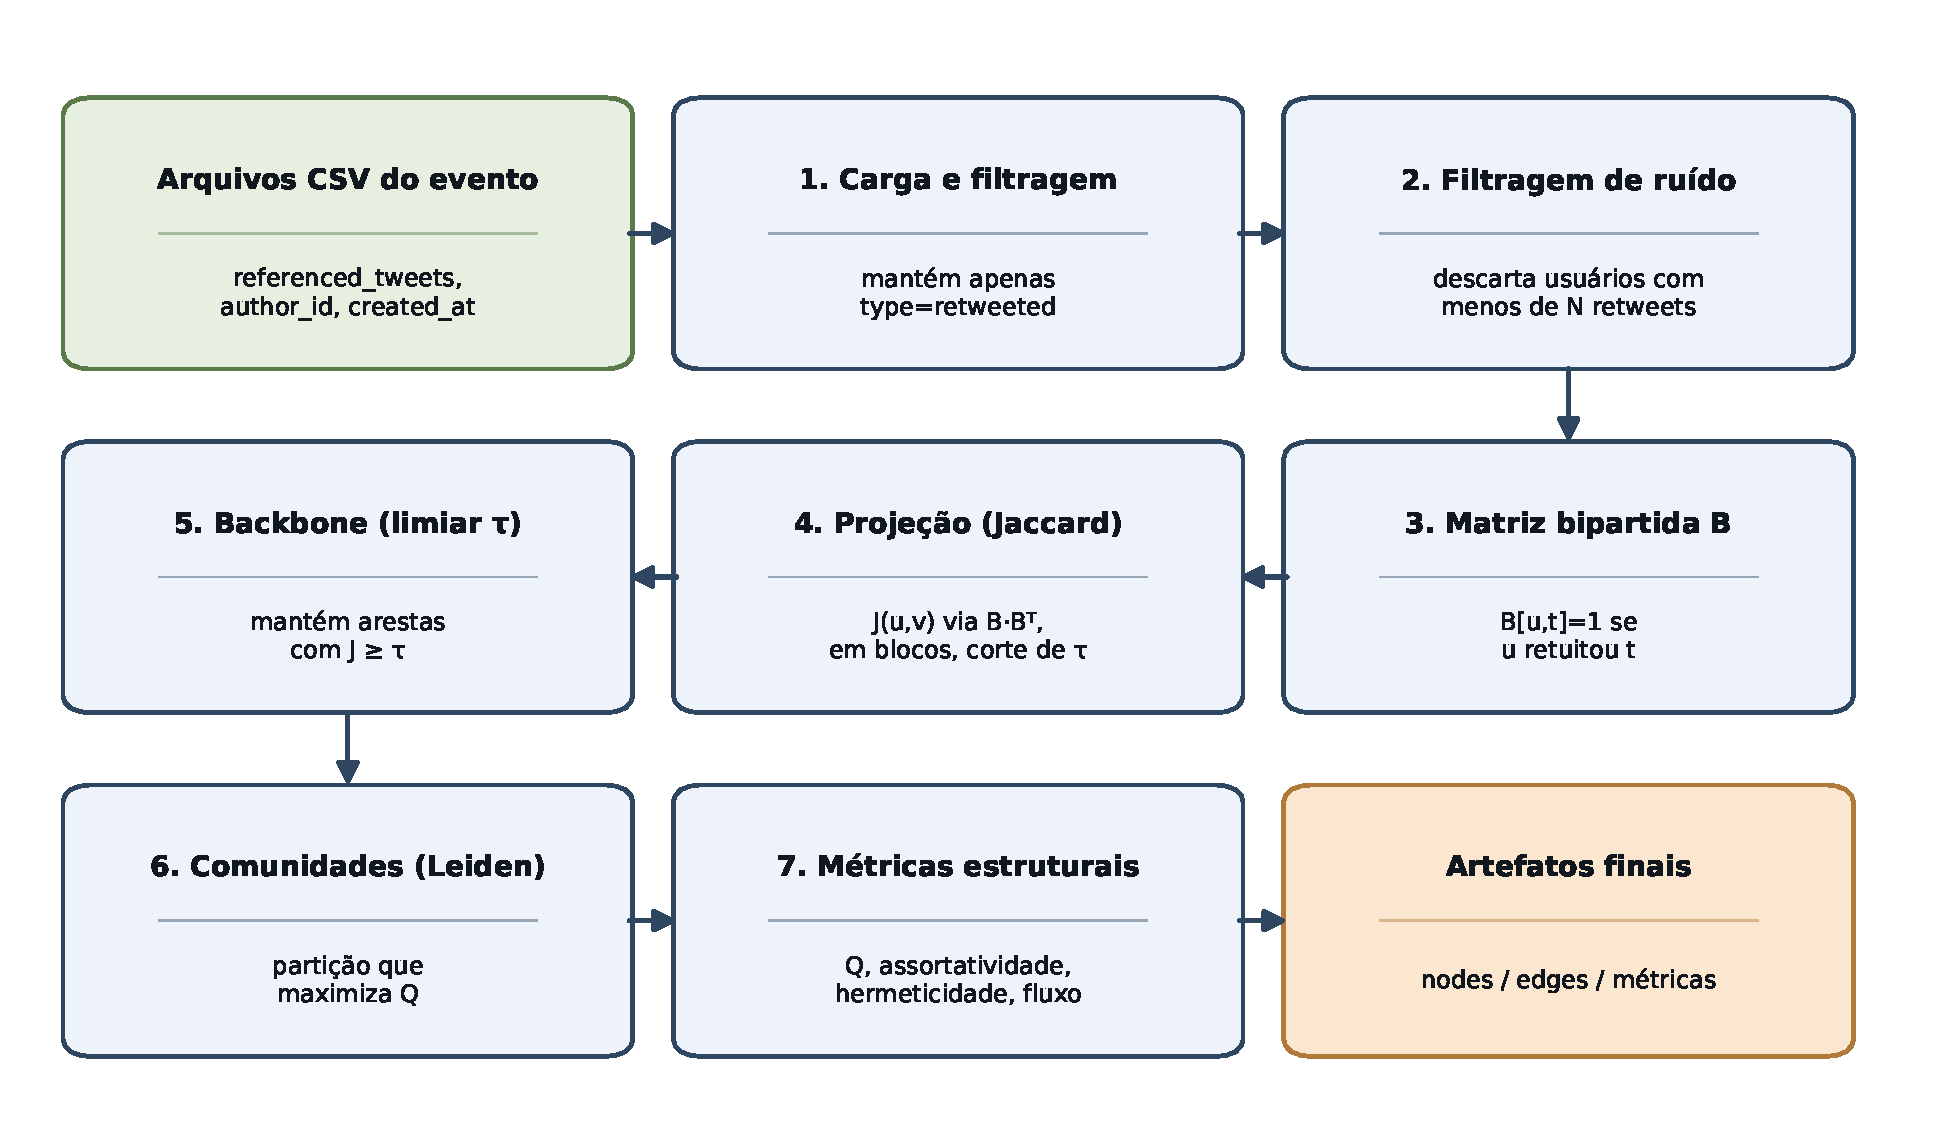
\includegraphics[width=0.96\textwidth]{fig_pipeline.pdf}
  \caption{Sequência de etapas da pipeline de construção e análise do grafo de co-retweet. A explosão combinatória de arestas causada por tweets de altíssimo alcance é tratada na etapa de projeção, com o corte de $\tau$ aplicado em blocos, e não por descarte de dados.}
  \label{fig:pipeline}
\end{figure*}

\subsection{Do dataset à estrutura de dados}
\label{sub:dataset}

Cada arquivo do dataset corresponde a um evento e contém, por registro, a data de criação, o identificador do autor da ação, o identificador da conversa e o campo \texttt{referenced\_tweets}. Esse último campo é o que organiza toda a construção. Quando vazio, indica um tweet original; quando preenchido, traz o tipo da referência (\texttt{retweeted}, \texttt{replied\_to} ou \texttt{quoted}) e o identificador do tweet referenciado. O primeiro passo da pipeline retém apenas os registros do tipo \texttt{retweeted}, descartando respostas, citações e originais, e produz um conjunto de pares (usuário, tweet retuitado).

É neste ponto que se materializa a restrição metodológica antecipada na revisão da literatura. O dataset preserva o identificador do tweet referenciado, mas não o seu autor. Reconstruir a rede de retweets dirigida no estilo de Conover et al. \cite{b_conover2011} e Interian e Rodrigues \cite{b_interian2023}, em que cada aresta liga o autor original ao usuário que o retuitou, exigiria recuperar o autor de cada tweet retuitado. Duas vias foram consideradas e descartadas. A recuperação por junção interna ao próprio dataset, cruzando tweets retuitados com tweets que aparecem como originais em algum arquivo, alcança apenas cerca de 19\% dos casos, taxa insuficiente para uma análise representativa. A recuperação por hidratação massiva via API, por sua vez, teria custo da ordem de centenas de dólares, incompatível com o orçamento do trabalho. A rede de co-retweet, descrita a seguir, dispensa o autor original e é a alternativa adotada. Sua justificativa conceitual, o acoplamento bibliográfico de Kessler \cite{b_kessler1963} aplicado a retweets, foi desenvolvida na Seção~\ref{sub:coretweet} do referencial.

A única filtragem de ruído aplicada antes da projeção descarta usuários que aparecem como retuitadores menos de $N$ vezes no evento. A justificativa é direta. Usuários com um ou dois retweets não fornecem sinal suficiente para serem associados de forma confiável a qualquer comunidade, e sua presença infla o grafo sem contribuir para a estrutura. Tweets de alto alcance não são filtrados, pois são o material central da análise narrativa prevista para a etapa posterior, e, do ponto de vista computacional, a explosão de arestas que provocam é tratada na projeção, não por descarte. O parâmetro $N$ é o mais sensível desta etapa e foi calibrado por evento, conforme discutido na Seção~\ref{sub:sensibilidade}.

\subsection{Construção do grafo de co-retweet}
\label{sub:construcao}

A partir dos pares (usuário, tweet), constrói-se uma matriz bipartida esparsa $B \in \{0,1\}^{|U| \times |T|}$, em que $U$ é o conjunto de usuários remanescentes e $T$ o conjunto de tweets retuitados ao menos uma vez no evento, com
\begin{equation}
B_{u,t} =
\begin{cases}
1, & \text{se o usuário } u \text{ retuitou o tweet } t,\\
0, & \text{caso contrário.}
\end{cases}
\end{equation}

A projeção sobre o lado dos usuários liga dois usuários que tenham retuitado ao menos um tweet em comum. O peso da aresta é o coeficiente de Jaccard sobre os conjuntos de tweets retuitados por cada um,
\begin{equation}
J(u,v) = \frac{|T_u \cap T_v|}{|T_u \cup T_v|},
\label{eq:jaccard}
\end{equation}
em que $T_u$ denota o conjunto de tweets retuitados pelo usuário $u$. O coeficiente varia de $0$, quando não há nenhum tweet em comum, a $1$, quando os dois usuários retuitaram exatamente o mesmo conjunto. A escolha do Jaccard em lugar da contagem absoluta de tweets em comum normaliza a similaridade pela atividade total de cada usuário, evitando que usuários hiperativos apareçam como artificialmente próximos de muitos outros apenas pelo volume de sua atividade.

O cálculo das interseções é feito por operações matriciais. O produto $B B^{\mathsf{T}}$ fornece, em cada posição $(u,v)$, a cardinalidade $|T_u \cap T_v|$, e a diagonal $|T_u|$ permite recuperar a união por inclusão-exclusão, $|T_u \cup T_v| = |T_u| + |T_v| - |T_u \cap T_v|$, de modo que a Equação~\eqref{eq:jaccard} é avaliada sem laço explícito sobre pares. O gargalo da operação não é o tempo de cálculo, mas o \emph{tamanho da saída}: um único tweet retuitado por dezenas de milhares de usuários gera, sozinho, um número quadrático de pares candidatos a aresta. Esse efeito é contido processando a projeção em blocos de usuários e aplicando o corte de limiar $\tau$ ainda dentro de cada bloco, antes de materializar a lista de arestas, o que mantém o uso de memória limitado independentemente do alcance dos tweets mais virais.

Convém registrar uma limitação do peso Jaccard sobre este objeto, que decorre da natureza do retweet. Como discutido no referencial, o retweet é um ato rápido e frequente, e o sinal que ele carrega é mais ruidoso que o de uma citação acadêmica. Em particular, um par de usuários de baixa atividade que compartilhe um único tweet viral recebe um Jaccard relativamente alto (no limite, dois usuários que retuitaram apenas aquele mesmo tweet têm $J=1$), ainda que a coincidência seja pouco informativa. Esse \emph{efeito de piso} é parte do motivo pelo qual se descartam usuários de pouquíssima atividade antes da projeção, e é também o que o limiar $\tau$ ajuda a atenuar ao remover as ligações mais fracas.

Após a projeção, aplica-se a extração de \emph{backbone} por limiar universal, retendo apenas as arestas com $J \ge \tau$. Adotou-se $\tau = 0{,}1$ de forma uniforme nos quatro eventos. O corte elimina ligações que conectam usuários com pouquíssima sobreposição entre dezenas de retweets cada, ligações que carregam pouca informação sobre proximidade real entre ambientes informacionais e que, se mantidas, produziriam um \emph{hairball} ilegível. A robustez dos achados a essa escolha é examinada na Seção~\ref{sub:sensibilidade}.

\subsection{Detecção de comunidades e métricas estruturais}
\label{sub:metricas}

Sobre o grafo resultante aplica-se o algoritmo de Leiden \cite{b_traag2019}, que busca uma partição dos nós maximizando a modularidade. A modularidade $Q$ mede o quanto a densidade de arestas dentro das comunidades supera a esperada em um grafo aleatório com a mesma distribuição de grau:
\begin{equation}
Q = \frac{1}{2m}\sum_{i,j}\left(A_{ij} - \frac{k_i k_j}{2m}\right)\delta(c_i,c_j),
\label{eq:modularidade}
\end{equation}
em que $A_{ij}$ é o peso da aresta entre $i$ e $j$, $k_i$ o grau ponderado de $i$, $m$ a soma dos pesos das arestas, $c_i$ a comunidade de $i$ e $\delta$ a função que vale $1$ quando $c_i = c_j$ e $0$ caso contrário.

A modularidade, contudo, não é diretamente comparável entre grafos de tamanhos e densidades distintos, pois é sensível ao número de nós e sofre de um limite de resolução conhecido. Como os quatro eventos diferem em escala e foram filtrados com $N$ distintos, a comparação entre eles não se apoia em $Q$, mas em duas quantidades normalizadas e interpretáveis. A primeira é a \emph{assortatividade nominal} por comunidade \cite{b_newman2003},
\begin{equation}
r = \frac{\sum_i e_{ii} - \sum_i a_i b_i}{1 - \sum_i a_i b_i},
\label{eq:assort}
\end{equation}
em que $e_{ij}$ é a fração de arestas entre as comunidades $i$ e $j$ e $a_i$, $b_i$ as somas marginais correspondentes. O coeficiente $r$ varia de $-1$ a $1$ e mede o quanto as arestas tendem a permanecer dentro das comunidades. A segunda é a \emph{hermeticidade} de cada comunidade, definida como a fração do peso de arestas que toca a comunidade $c$ e permanece interna a ela,
\begin{equation}
h_c = \frac{I_c}{I_c + E_c},
\label{eq:herm}
\end{equation}
em que $I_c$ é o peso das arestas internas a $c$ e $E_c$ o peso das arestas que ligam $c$ ao resto do grafo. A hermeticidade varia de $0$ a $1$ e é normalizada pelo volume de cada comunidade, o que a torna comparável entre comunidades de tamanhos diferentes e entre eventos, e responde diretamente à segunda pergunta da introdução, sobre o \emph{grau} de fechamento de cada lado.

Complementarmente, computa-se a \emph{matriz de fluxo} entre as comunidades dominantes, definidas como aquelas que reúnem ao menos $1\%$ dos nós. Cada célula registra a fração do peso total das arestas que cai dentro de uma comunidade (na diagonal) ou entre um par delas (fora da diagonal). Por construção sobre um grafo não dirigido, a matriz é simétrica, e a soma da diagonal com o triângulo superior recupera a totalidade do peso. A leitura dessa matriz permite verificar se as comunidades dominantes se agregam em blocos maiores. Definindo como \emph{super-polos} os componentes conexos do grafo de comunidades em que se mantêm apenas os pares com fluxo mútuo acima de $1\%$ do peso total, obtém-se uma descrição da macroestrutura que é robusta à fragmentação fina das comunidades.

\subsection{Resultados estruturais}
\label{sub:resultados}

A pipeline foi aplicada aos quatro eventos com $\tau = 0{,}1$ e com o filtro $N$ calibrado por evento. A Tabela~\ref{tab:mestre} resume as métricas obtidas, e a Figura~\ref{fig:grafos} apresenta os grafos renderizados, coloridos por comunidade. Os parâmetros de filtragem são declarados na tabela, com $N$ menor nos eventos de menor volume, para não dizimar o grafo, e o mesmo $\tau$ em todos, de modo a não introduzir, pela seleção de arestas, diferenças nas próprias métricas que se deseja comparar.

\begin{table*}[tbp]
  \centering
  \caption{Métricas estruturais por evento. $h^\star$ é a hermeticidade do polo mais fechado e ``\% polo'' o seu tamanho relativo. ``Pol.'' é o número de super-polos (componentes do grafo de comunidades com fluxo mútuo $>1\%$).}
  \label{tab:mestre}
  \setlength{\tabcolsep}{4pt}
  \begin{tabular}{lccrcccccc}
    \toprule
    Evento & $N$ & $\tau$ & N\'os & Ar. & $Q$ & $r$ & $h^\star$ & \% polo & Pol. \\
    \midrule
    Mobiliza\c{c}\~ao & 3 & 0{,}10 & 16\,495 & 9{,}3M & 0{,}471 & 0{,}686 & 0{,}969 & 45{,}6 & 2 \\
    R. Jefferson      & 8 & 0{,}10 & 27\,042 & 32{,}5M & 0{,}308 & 0{,}507 & 0{,}999 & 59{,}1 & 2 \\
    Elei\c{c}\~oes    & 5 & 0{,}10 & 9\,742  & 14{,}3M & 0{,}149 & 0{,}168 & 0{,}979 & 3{,}4  & 2 \\
    Invas\~ao         & 7 & 0{,}10 & 33\,305 & 12{,}0M & 0{,}498 & 0{,}745 & 0{,}999 & 44{,}2 & 2 \\
    \bottomrule
  \end{tabular}
\end{table*}

\begin{figure*}[tbp]
  \centering
  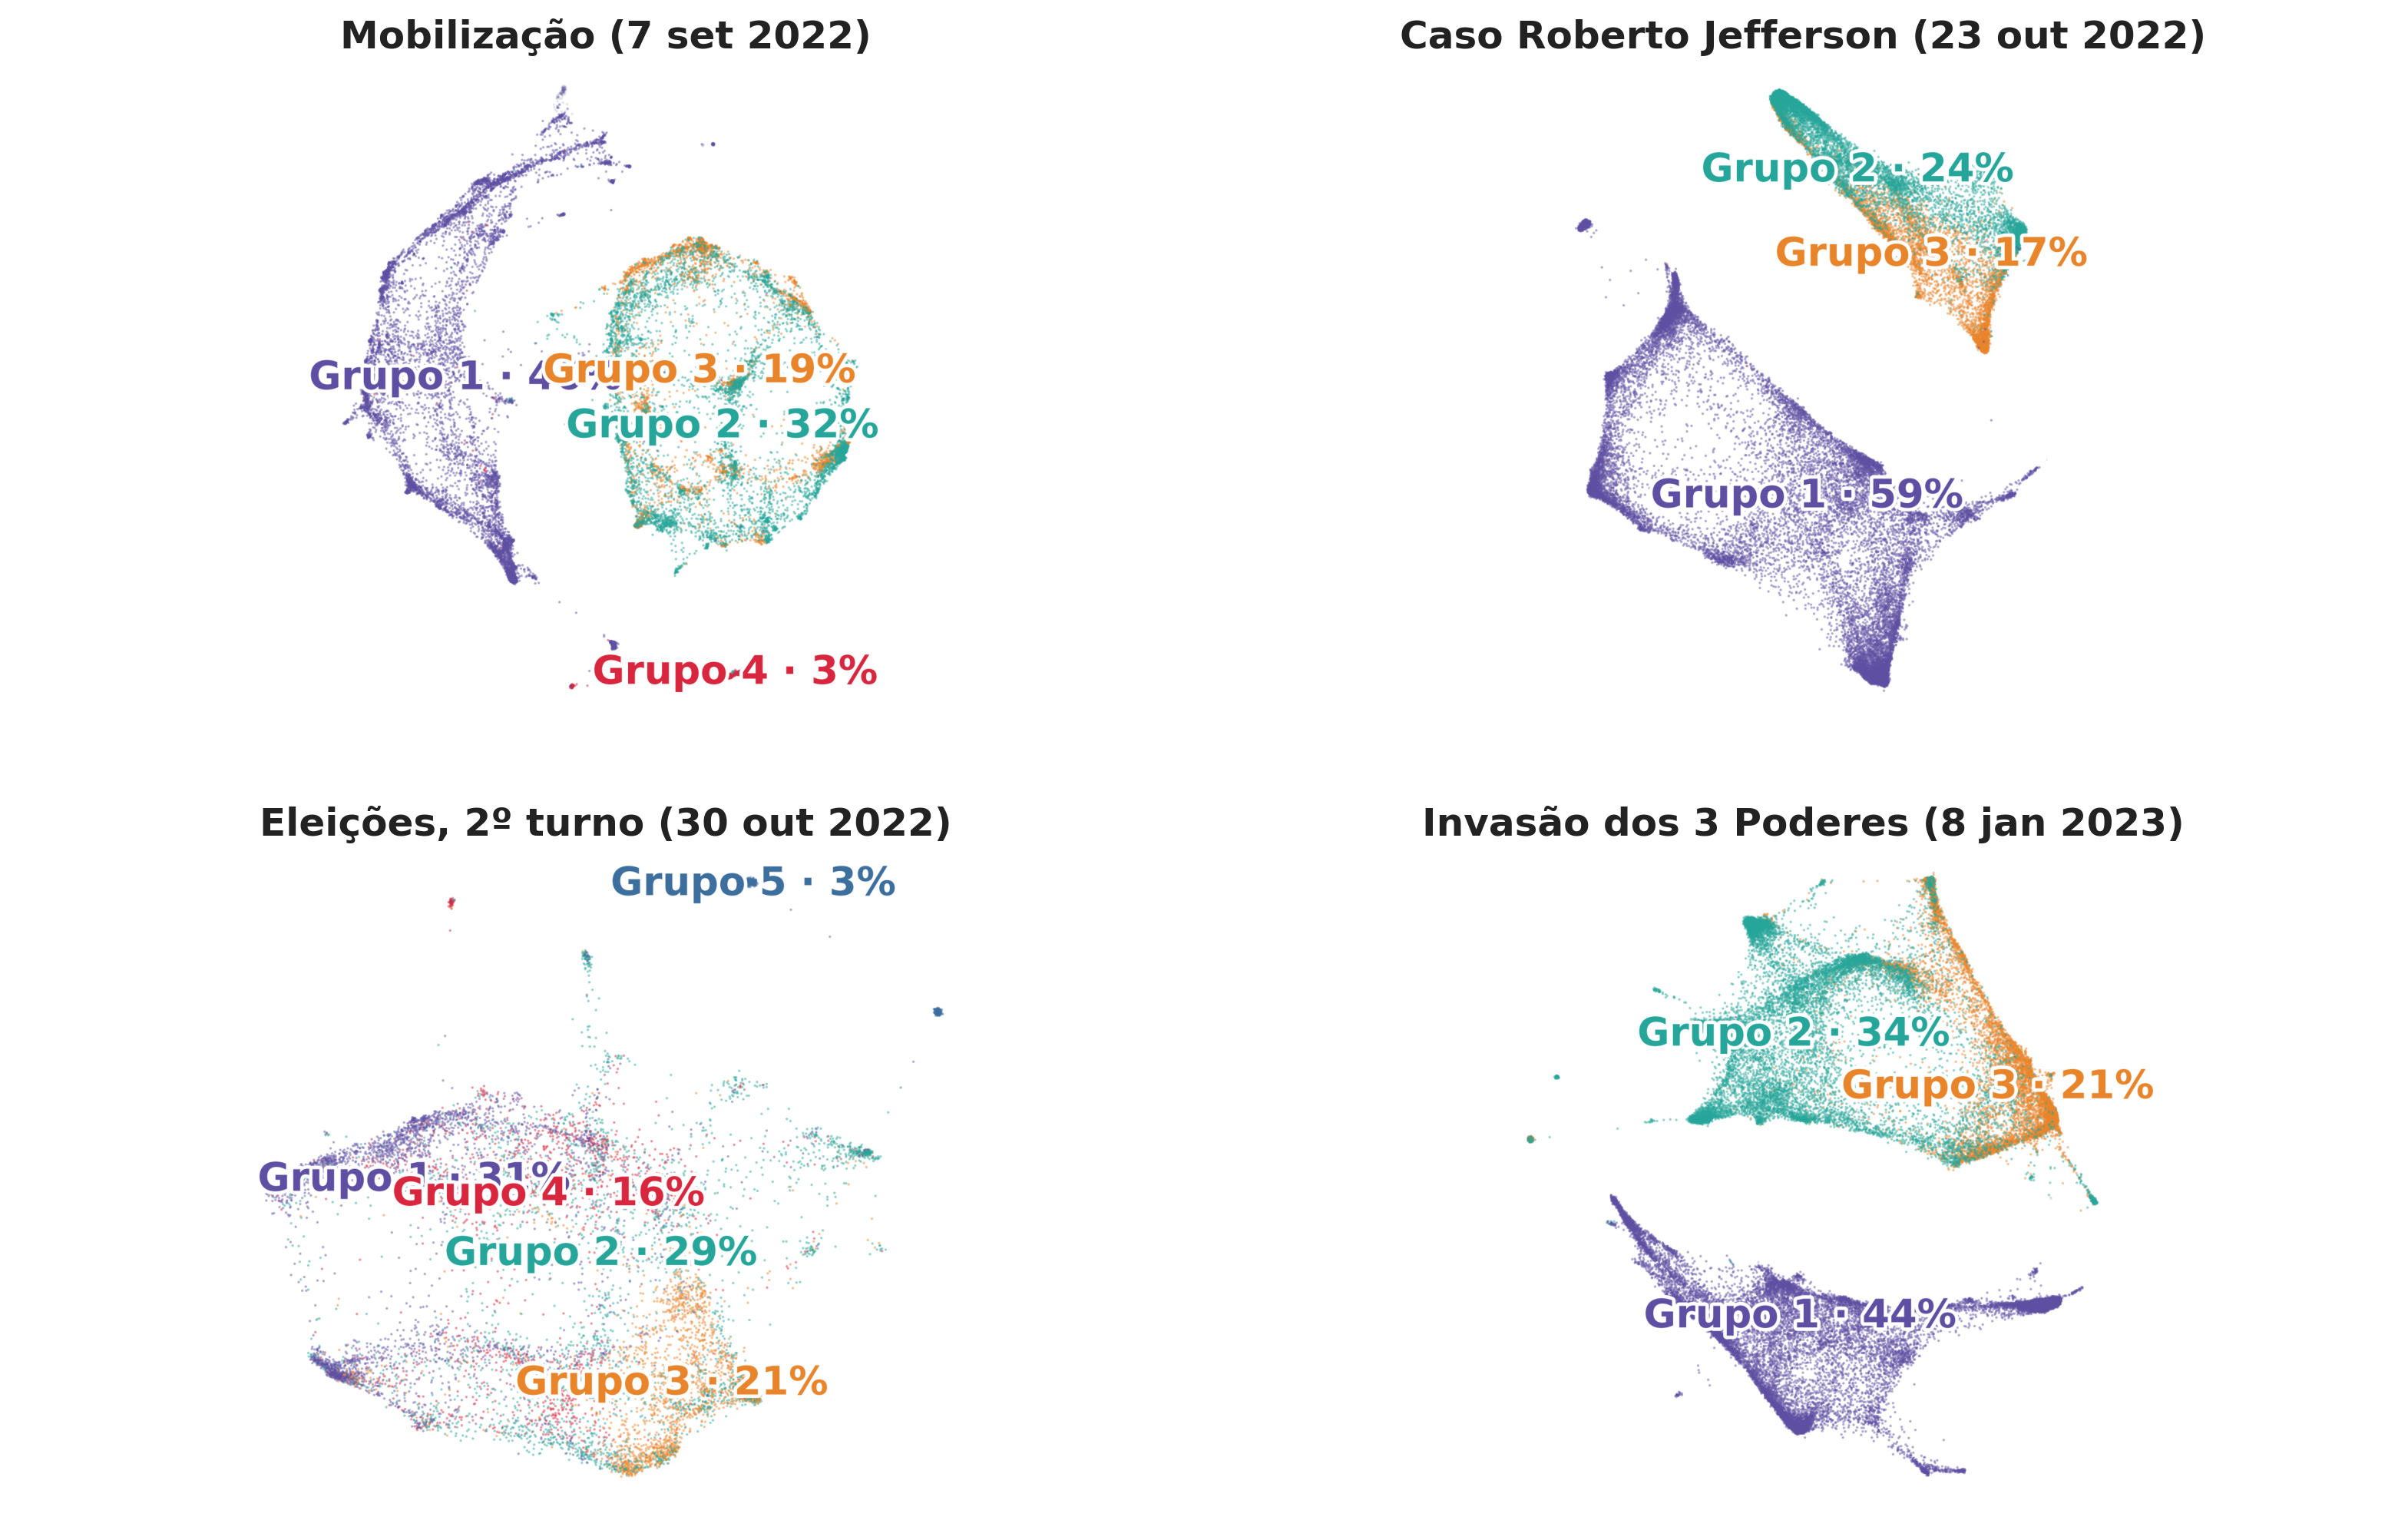
\includegraphics[width=\textwidth]{fig_grafos_drl.png}
  \caption{Grafos de co-retweet dos quatro eventos, em layout dirigido por força (DRL). Cada ponto é um usuário, a proximidade entre pontos reflete a quantidade de retweets em comum e a cor indica a comunidade. A porcentagem ao lado de cada rótulo é a parcela de usuários do evento naquele grupo. Nos três flashpoints (mobilização, Roberto Jefferson e invasão), um polo aparece nitidamente destacado do restante. No dia do segundo turno, a separação se desfaz em uma massa única.}
  \label{fig:grafos}
\end{figure*}

\subsubsection{Existem dois campos, e um deles é hermético}

Em três dos quatro eventos, a mobilização do 7 de setembro, o caso Roberto Jefferson e a invasão de 8 de janeiro, a estrutura é a mesma, e responde às duas primeiras perguntas da introdução de uma só vez. Existe sempre uma comunidade dominante praticamente lacrada, com hermeticidade entre $0{,}97$ e $0{,}999$, ao lado de um conjunto de comunidades porosas que trocam peso entre si de forma intensa. A matriz de fluxo da invasão de 8 de janeiro ilustra o padrão de modo nítido: o polo lacrado (Grupo~1) troca com cada um dos outros dois grupos apenas $0{,}024\%$ e $0{,}015\%$ do peso total da rede, ao passo que os dois grupos porosos (Grupos~2 e 3) trocam entre si $16{,}5\%$. Em termos de hermeticidade, o polo lacrado atinge $0{,}999$, contra $0{,}55$ e $0{,}62$ dos demais. O mesmo desenho aparece na mobilização e em Roberto Jefferson, como mostra a Figura~\ref{fig:hermeticidade}. Em cada um desses eventos, uma comunidade ampla, de $45$ a $59\%$ dos usuários, se fecha quase por completo, enquanto o restante se distribui em comunidades que se interpenetram.

A detecção de super-polos confirma que, abaixo da fragmentação fina, a macroestrutura desses três eventos é bipolar: as comunidades dominantes se agregam em exatamente dois blocos, sempre na forma \{polo lacrado\} \emph{versus} \{restante poroso\}. É esse achado que converge, por um caminho metodológico independente, com o de Interian e Rodrigues \cite{b_interian2023}. Enquanto aqueles autores, sobre uma rede de retweets dirigida do período eleitoral, encontram uma comunidade marcadamente mais isolada e coesa que as demais, a rede de co-retweet aqui construída encontra, em torno de cada flashpoint, um polo cujo fechamento é praticamente total. A convergência é estrutural, não ideológica: a presente etapa identifica \emph{uma} comunidade hermética, sem ainda afirmar a que orientação política ela corresponde.

\begin{figure*}[tbp]
  \centering
  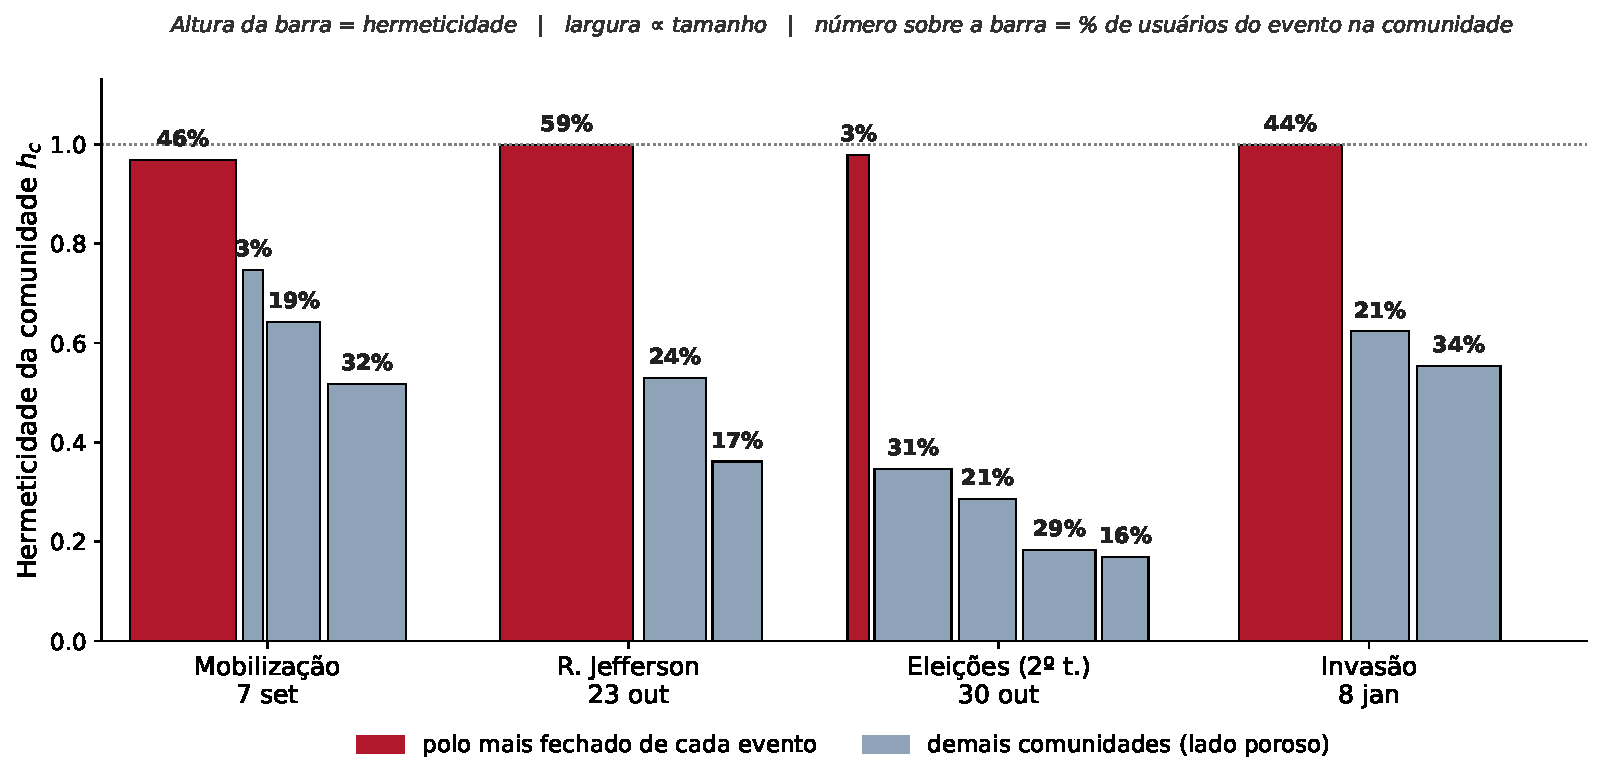
\includegraphics[width=0.92\textwidth]{fig_hermeticidade.pdf}
  \caption{Hermeticidade das comunidades dominantes em cada evento. A altura da barra é a hermeticidade $h_c$, a largura é proporcional ao tamanho da comunidade e o número sobre a barra é a parcela de usuários do evento naquele grupo. Nos três flashpoints, o polo mais fechado (em vermelho) é amplo e quase totalmente selado. No evento das eleições, ele se reduz a um enclave de $3{,}4\%$, e as demais comunidades têm fechamento baixo e semelhante entre si.}
  \label{fig:hermeticidade}
\end{figure*}

\subsubsection{O dia da eleição é a exceção reveladora}

O quarto evento, o dia do segundo turno, não reproduz o padrão dos demais, e é justamente por isso que ele importa para a terceira pergunta da introdução, sobre a forma da divisão. Sua modularidade é $0{,}149$, contra $0{,}471$ a $0{,}498$ dos flashpoints, e sua assortatividade é de apenas $0{,}168$. Não há um polo lacrado dominante. O único enclave fortemente fechado reúne $3{,}4\%$ dos usuários, e a maior parte da rede forma uma massa porosa em que quatro comunidades trocam peso umas com as outras sem fronteiras nítidas (Figura~\ref{fig:hermeticidade}, terceiro grupo). O grafo correspondente, na Figura~\ref{fig:grafos}, é visivelmente menos segregado que os demais.

Para verificar se essa ausência de estrutura é real ou artefato do limiar adotado, variou-se $\tau$ no evento das eleições (Figura~\ref{fig:tau}). A modularidade só alcança valores comparáveis aos dos flashpoints quando o limiar é elevado a $0{,}3$ ou $0{,}4$, ou seja, quando se exige uma sobreposição de retweets muito alta para que dois usuários permaneçam ligados. No limiar de comparação $\tau = 0{,}1$, comum a todos os eventos, a rede do segundo turno é um \emph{hairball}: a estrutura existe, mas está soterrada sob uma profusão de ligações fracas e transversais. A leitura proposta é que o dia da eleição inunda a rede de conteúdo amplamente compartilhado (o ato de votar, os resultados e as reações imediatas), material que atravessa as fronteiras políticas e que, no co-retweet, aproxima usuários de lados opostos. O momento de maior participação comum é, em termos de co-retweet, o de menor segregação.

Esse contraste tem um valor metodológico que convém explicitar. Se a pipeline produzisse comunidades herméticas em qualquer entrada, o achado dos três flashpoints seria suspeito de ser um artefato do método. O fato de o mesmo procedimento, aplicado ao dia da eleição com os mesmos parâmetros, não produzir um polo lacrado dominante indica que o fechamento observado nos demais eventos é uma propriedade dos dados, e não uma imposição da metodologia.

\begin{figure}[tbp]
  \centering
  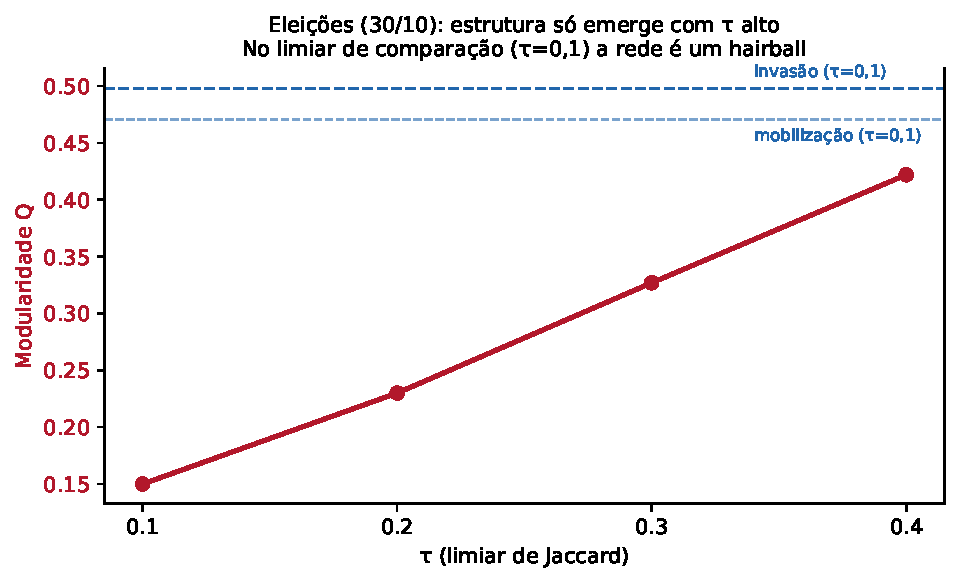
\includegraphics[width=0.96\columnwidth]{fig_tau_eleicoes.pdf}
  \caption{Eleições (30/10): modularidade em função do limiar $\tau$. A estrutura só emerge sob cortes agressivos. No limiar de comparação ($\tau = 0{,}1$), o evento permanece muito abaixo dos flashpoints (linhas tracejadas).}
  \label{fig:tau}
\end{figure}

\subsubsection{Os dois lados não têm o mesmo formato}

A terceira pergunta da introdução, sobre se os dois lados da divisão têm o mesmo formato, recebe dos quatro eventos uma resposta negativa consistente. Em nenhum deles a estrutura é a de dois blocos espelhados. Nos flashpoints, um polo se fecha quase por completo enquanto o lado oposto permanece poroso e, com frequência, subdividido em mais de uma comunidade que troca peso livremente. Essa assimetria de fechamento, e não o valor absoluto da modularidade, é a constante estrutural do arco, e ela ecoa a polarização assimétrica já documentada para o Twitter político brasileiro por Soares, Recuero e Zago \cite{b_soares2019} e por Recuero, Soares e Zago \cite{b_recuero2021}. Vale notar ainda que o tamanho do polo lacrado varia entre os eventos, de $45$ a $59\%$ nos flashpoints e apenas $3{,}4\%$ nas eleições, o que mostra que ``estar fechado'' e ``ser maioria'' são propriedades independentes: o fechamento de uma comunidade não é função do seu tamanho.

\subsection{Análise de sensibilidade}
\label{sub:sensibilidade}

Como o filtro $N$ varia entre eventos, é necessário verificar que os achados não dependem dessa escolha. Para o evento de 8 de janeiro, variou-se $N$ de $5$ a $20$ com $\tau$ fixo (Figura~\ref{fig:sensN}). A modularidade permanece em torno de $0{,}49$ ao longo de toda a faixa, oscilando menos de $0{,}03$ enquanto o número de nós varia de $48$ mil a $9$ mil. Mais importante, o número de super-polos permanece igual a $2$ em todos os valores de $N$, o que indica que a macroestrutura bipolar é invariante ao filtro, ainda que o número de comunidades em que o lado poroso se fragmenta dependa dele. Disso decorre a postura adotada na comparação entre eventos. O achado qualitativo, a bipolaridade assimétrica nos flashpoints e sua ausência no dia da eleição, é robusto ao parâmetro e pode ser comparado entre eventos filtrados com $N$ distintos. Os valores numéricos específicos de $Q$ e de hermeticidade, por outro lado, são tratados como descritores internos de cada evento, e não como uma série temporal a ser lida como tendência.

Quanto ao limiar de \emph{backbone}, a opção por um $\tau$ comum a todos os eventos foi deliberada. Em uma versão anterior, o evento Roberto Jefferson havia sido processado com $\tau = 0{,}15$ por restrição de memória. A reexecução com $\tau = 0{,}1$, embora tenha mais que dobrado o número de arestas, manteve a hermeticidade do polo lacrado em $0{,}999$, praticamente idêntica à da versão anterior. O fechamento, portanto, não era um efeito do limiar.

\begin{figure}[tbp]
  \centering
  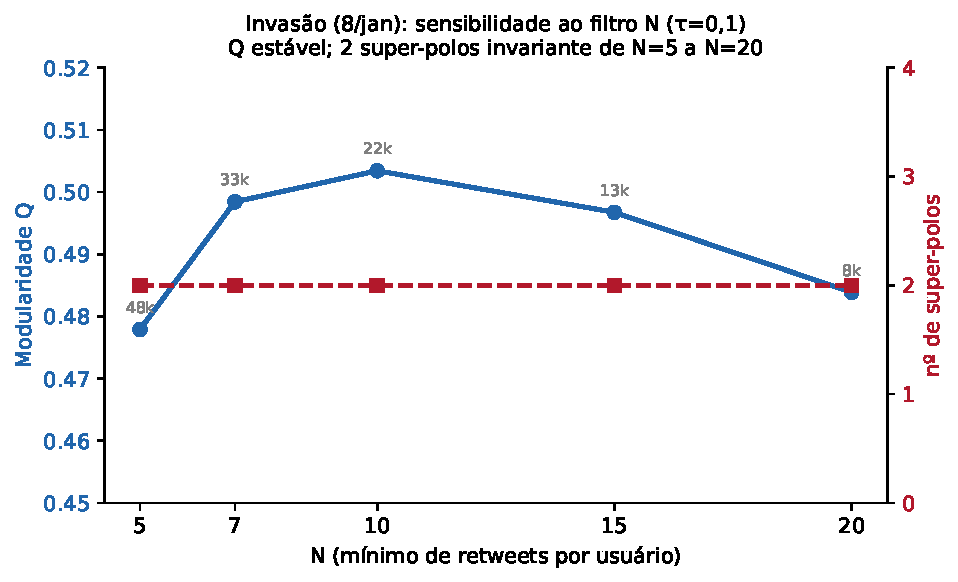
\includegraphics[width=0.96\columnwidth]{fig_sensibilidade_N.pdf}
  \caption{Invasão (8/jan): sensibilidade ao filtro $N$, com $\tau = 0{,}1$ fixo. A modularidade é estável e o número de super-polos permanece igual a $2$ de $N=5$ a $N=20$, o que indica que a macroestrutura bipolar não depende do filtro.}
  \label{fig:sensN}
\end{figure}

\subsection{Síntese: o que a estrutura mostra e o que ela não mostra}
\label{sub:sintese}

A etapa relatada estabelece, com base nos dados, três fatos estruturais. Primeiro, em torno dos eventos contenciosos analisados, a rede de co-retweet se organiza de forma bipolar, com um polo praticamente lacrado oposto a um lado poroso. Segundo, esse fechamento é fortemente assimétrico, de modo que os dois lados da divisão não têm o mesmo formato. Terceiro, a segregação não é constante ao longo do arco. O dia da eleição, momento de participação compartilhada, é o de menor polarização de co-retweet, o que serve simultaneamente de contraste substantivo e de controle metodológico contra a suspeita de que o método produza fechamento artificialmente.

É igualmente importante delimitar o que esta etapa não demonstra. A rede de co-retweet mede similaridade de consumo informacional, não fluxo de influência, e as comunidades aqui detectadas são, por ora, objetos estritamente estruturais: comunidades discursivas, no sentido de Becatti et al. \cite{b_becatti2019}, e não campos ideológicos identificados. A pergunta central do trabalho, sobre como dois grupos constroem leituras divergentes de um mesmo fato, exige caracterizar o \emph{conteúdo} amplificado por cada comunidade, o que está fora do alcance de uma análise puramente estrutural e constitui o objeto da etapa seguinte. O que esta contribuição entrega é a pré-condição dessa investigação: a demonstração de que as comunidades existem, de que uma delas se fecha de modo quase total e de que essa configuração se repete, com forma reconhecível, ao longo do arco que conduz ao 8 de janeiro.

\begin{thebibliography}{00}
\bibitem{b_recuero2021} R. Recuero, F. B. Soares, and G. Zago, ``Polarização, hiperpartidarismo e câmaras de eco: como circula a desinformação sobre Covid-19 no Twitter,'' Contracampo, vol. 40, no. 1, 2021.
\bibitem{b_axfors2021} C. Axfors et al., ``Mortality outcomes with hydroxychloroquine and chloroquine in COVID-19 from an international collaborative meta-analysis of randomized trials,'' Nature Communications, vol. 12, no. 1, art. 2349, 2021.
\bibitem{b_singh2020} S. K. Singh, A. Ravindran, and B. K. Patel, ``No benefit of hydroxychloroquine in COVID-19: Results of systematic review and meta-analysis of randomized controlled trials,'' Diabetes \& Metabolic Syndrome: Clinical Research \& Reviews, vol. 14, no. 5, pp. 1419--1423, 2020.
\bibitem{b_watson2022} O. J. Watson et al., ``Global impact of the first year of COVID-19 vaccination: a mathematical modelling study,'' The Lancet Infectious Diseases, vol. 22, no. 9, pp. 1293--1302, 2022.
\bibitem{b_interian2023} R. Interian and F. A. Rodrigues, ``Group polarization, influence, and domination in online interaction networks: A case study of the 2022 Brazilian elections,'' arXiv preprint arXiv:2303.16859, 2023.
\bibitem{b_pariser2011} E. Pariser, The Filter Bubble: How the New Personalized Web Is Changing What We Read and How We Think. New York: Penguin Press, 2011.
\bibitem{b_sunstein2001} C. R. Sunstein, Echo Chambers: Bush v. Gore, Impeachment, and Beyond. Princeton, NJ: Princeton Univ. Press, 2001.
\bibitem{b_conover2011} M. D. Conover, B. Gonçalves, J. Ratkiewicz, A. Flammini, and F. Menczer, ``Predicting the political alignment of Twitter users,'' in Proc. 2011 IEEE 3rd Int. Conf. Privacy, Security, Risk and Trust and 2011 IEEE 3rd Int. Conf. Social Computing, 2011, pp. 192--199.
\bibitem{b_soares2019} F. B. Soares, R. Recuero, and G. Zago, ``Asymmetric polarization on Twitter and the 2018 Brazilian presidential elections,'' in Proc. 10th Int. Conf. Social Media and Society (SMSociety), 2019, pp. 67--76.
\bibitem{b_kessler1963} M. M. Kessler, ``Bibliographic coupling between scientific papers,'' American Documentation, vol. 14, no. 1, pp. 10--25, 1963.
\bibitem{b_becatti2019} A. Becatti, G. Caldarelli, R. Lambiotte, and F. Saracco, ``Extracting significant signal of news consumption from social networks: the case of Twitter in Italian political elections,'' Applied Network Science, vol. 4, art. 62, 2019.
\bibitem{b_rocha2024} I. Rocha, ``Persistent Homology generalizations for Social Media Network Analysis,'' arXiv preprint arXiv:2404.19257, 2024.
\bibitem{b_cicchini2022} T. Cicchini, S. M. del Pozo, E. Tagliazucchi, and P. Balenzuela, ``News sharing on Twitter reveals emergent fragmentation of media agenda and persistent polarization,'' EPJ Data Science, vol. 11, no. 1, art. 48, 2022.
\bibitem{b_silva2024} L. J. Silva et al., ``Tweet\_Eleições\_2022: um dataset de tweets durante as eleições presidenciais brasileiras de 2022,'' Zenodo, 2024, doi: 10.5281/zenodo.11206577.
\bibitem{b_traag2019} V. A. Traag, L. Waltman, and N. J. van Eck, ``From Louvain to Leiden: guaranteeing well-connected communities,'' Scientific Reports, vol. 9, no. 1, art. 5233, 2019.
\bibitem{b_newman2003} M. E. J. Newman, ``Mixing patterns in networks,'' Physical Review E, vol. 67, no. 2, art. 026126, 2003.
\end{thebibliography}

\end{document}
